The component SmartLogisticsRefboxServer has not changed during the implementation process. Therefor this chapter also just summarizes the functionality of the component and it is again recommended to read the Technical Report of 2017 for more specific information.

\subsubsection{Overview}

The component handles the communication between the physical Refbox and the robots. The Refbox uses Google Protocol-Buffers for message serialization. Therefor a component is introduced to act as an interface between the physical Refbox and the robots on the field. The task of the component is to receive Google Protocol-Buffers messages from the Refbox and map them into TCL-messages of Smartsoft. Then it sends the TCL-message to the InstructionPlanner for further processing. 

\begin{figure}[!h]
\centering
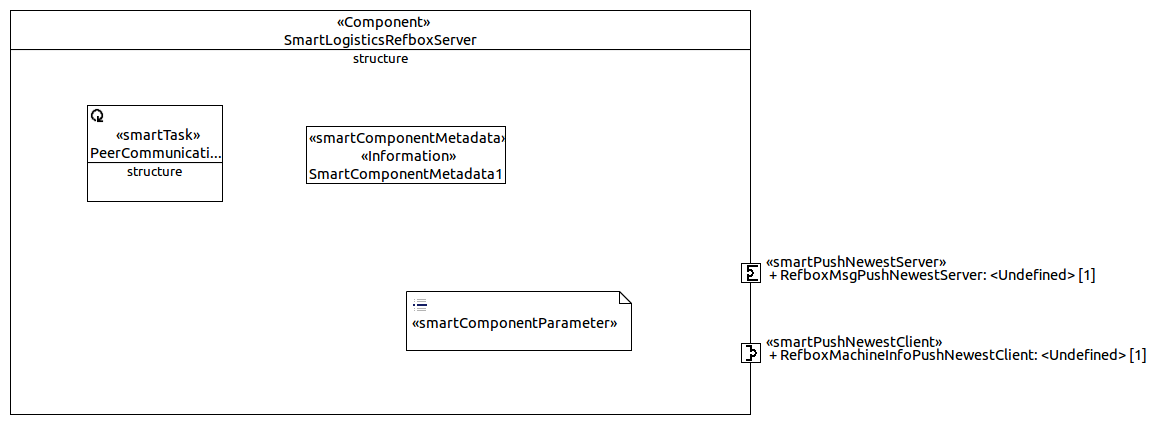
\includegraphics[width=\linewidth]{pic/component_refbox_server.png}
\caption{Model of Refbox server}
\label{fig:modelRefboxServer}
\end{figure}


\subsubsection{Configuration}

The component can be modified by the following parameters:
\begin{itemize}
\item \textbf{HostIP}, the IP address of the Referee Box
\item \textbf{Name}, the name of the robot, which is displayed on the Referee Box GUI
\item \textbf{Number}, the number of the robot, which is displayed on the Referee Box GUI
\item \textbf{Cryptokey} the key, which is used for the encrypted team channel
\end{itemize}

At the Robocup competition 2017 the hosts used AES with Electronic Codebook Encryption (ECB), while the Refbox in the laboratory used Cipher Block Chaining (CBC) for encryption. Therefor the team has to change the cipher method to the correct version at the competition.